
\documentclass[a4paper, 12pt]{article}

\usepackage{graphicx}
\usepackage{longtable}

\begin{document}
\title{ARE213 Problem Set \#1A}
\author{Peter Alstone \& Frank Proulx}
\maketitle

\section{Problem \#1}
\subsection{Part A}

Data records are excluded from the dataset based whether the following variables take the noted values \(as found in the data manual\):

\subsection{Part B}
We dropped all rows where any data were missing in that row.  One way that the data cleaning process could be improved would be to only remove records based on the variables of interest (as are determined in subsequent analysis) since missing values in fields that are not eventually used in the analysis do not pose a problem..  This would result in a more iterative approach, however, and increase workload on the researcher.

We used some exploratory analysis to understand if the records that were dropped due to missing data \textit{somewhere} in the record were representative.  First we compared a few simple summary statistics between the "full record" and "partial record" data on variables of interest for this analysis.  These are summarized in Table \ref{tab:compareMissingData}.  Better APGAR scores and lower incidence of smoking may be correlated with having full datasets, which indicates the people who have missing data may bias the sample.  We also used agnostic linear regression to understand the relationship between the presence of full records and three key variables: one-minute apgar (omaps), five-minute apgar (fmaps), and number of cigarettes smoked each day (cigar).  The results summarized in Table \ref{tab:lmMissingData} indicate there is statistical significance in each of the factors (i.e. all three are useful predictors for whether a person has a full data record) but also that the influence of the factors is small.  Figure \ref{fig:cigarFullData} shows the distribution in the number of cigarettes smoked by those with and without full records.  The distribution of values is basically the same (clusters around multiples of five up to 20, or, a "pack a day") between the two datasets.  

Overall, in spite of the bias from removing heavier smokers with lower apgar scores from the data, the overall number removed is relatively small and the size of the bias (indicated by the coefficients in the linear model) is relatively small.  

% Table created by stargazer v.4.0 by Marek Hlavac, Harvard University. E-mail: hlavac at fas.harvard.edu
% Date and time: Thu, Sep 19, 2013 - 16:27:57
\begin{table}[!htbp] \centering 
  \caption{Comparison of data with full records to those with missing data across key variables} 
  \label{tab:compareMissingData} 
\begin{tabular}{@{\extracolsep{5pt}} ccccccc} 
\\[-1.8ex]\hline 
\hline \\[-1.8ex] 
full.record & mean.omaps & sd.omaps & mean.fmaps & sd.fmaps & mean.cigar & sd.cigar \\ 
\hline \\[-1.8ex] 
FALSE & $7.905$ & $1.572$ & $8.880$ & $1.030$ & $3.945$ & $7.422$ \\ 
TRUE & $8.117$ & $1.260$ & $9.009$ & $0.707$ & $1.907$ & $5.297$ \\ 
\hline \\[-1.8ex] 
\normalsize 
\end{tabular} 
\end{table} 


% Table created by stargazer v.4.0 by Marek Hlavac, Harvard University. E-mail: hlavac at fas.harvard.edu
% Date and time: Thu, Sep 19, 2013 - 16:32:14
\begin{table}[!htbp] \centering 
  \caption{Linear model results for predicting whether full records are present based on selected variable of interest in the dataset} 
  \label{tab:lmMissingData} 
\begin{tabular}{@{\extracolsep{5pt}}lc} 
\\[-1.8ex]\hline 
\hline \\[-1.8ex] 
 & \multicolumn{1}{c}{\textit{Dependent variable:}} \\ 
\cline{2-2} 
\\[-1.8ex] & full.record \\ 
\hline \\[-1.8ex] 
 omaps & 0.002$^{***}$ \\ 
  & (0.001) \\ 
  & \\ 
 fmaps & 0.007$^{***}$ \\ 
  & (0.001) \\ 
  & \\ 
 cigar & $-$0.003$^{***}$ \\ 
  & (0.0001) \\ 
  & \\ 
 Constant & 0.882$^{***}$ \\ 
  & (0.007) \\ 
  & \\ 
\hline \\[-1.8ex] 
Observations & 119,384 \\ 
R$^{2}$ & 0.007 \\ 
Adjusted R$^{2}$ & 0.007 \\ 
Residual Std. Error & 0.195 \\ 
F Statistic & 276.305 \\ 
\hline 
\hline \\[-1.8ex] 
\textit{Note:}  & \multicolumn{1}{r}{$^{*}$p$<$0.1; $^{**}$p$<$0.05; $^{***}$p$<$0.01} \\ 
\normalsize 
\end{tabular} 
\end{table}


\begin{figure}[!h] %  figure placement: here, top, bottom, or page
   \centering
   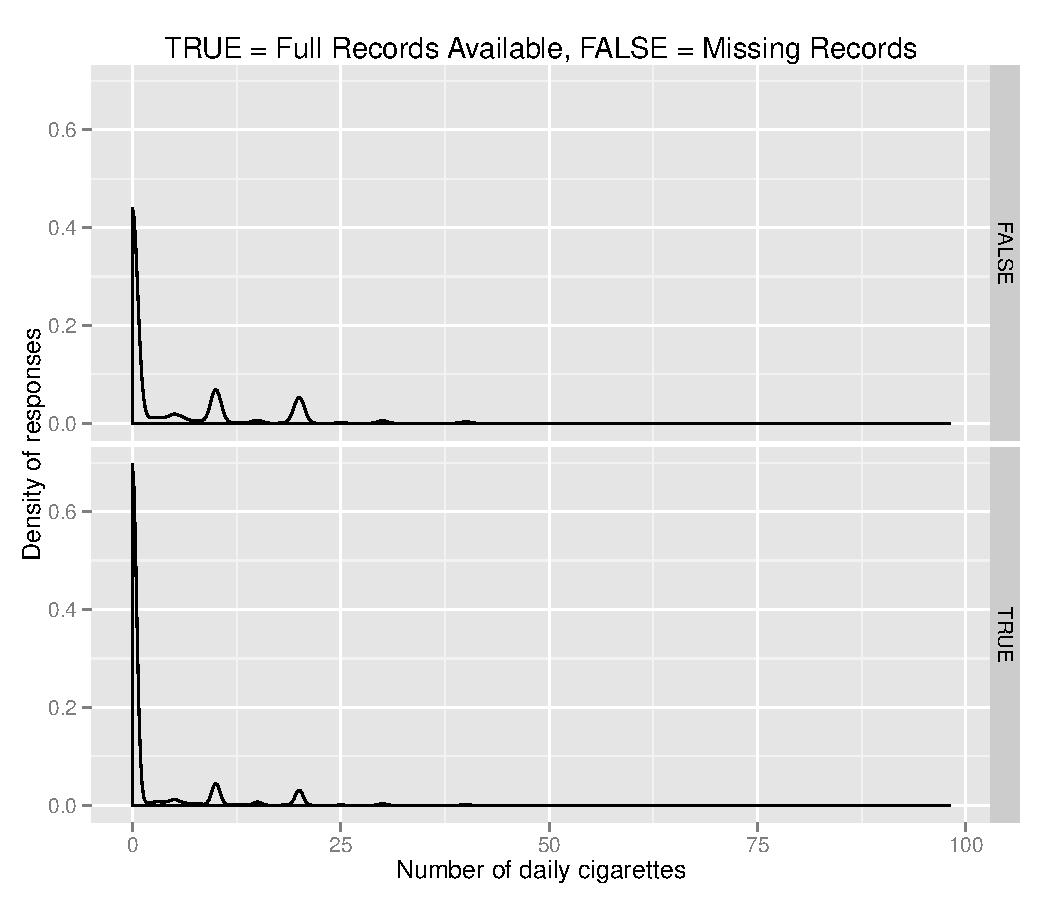
\includegraphics[width=4in]{img/cigar-by-record-type.pdf} 
   \caption{Cigarette use rate by presence of full data record.}
   \label{fig:cigarFullData}
\end{figure}

\subsection{Part C}
The summary table for the remaining data after cleaning is below.
% Code for the summary table from file summarytable.tex starts here...
% latex.default(summarytable) 
%

% Table created by stargazer v.4.0 by Marek Hlavac, Harvard University. E-mail: hlavac at fas.harvard.edu
% Date and time: Fri, Sep 20, 2013 - 11:30:46
\begin{table}[!htbp] \centering 
  \caption{Summary for cleaned dataset} 
  \label{tab:cleanSummary} 
\begin{tabular}{@{\extracolsep{5pt}}lccccc} 
\\[-1.8ex]\hline 
\hline \\[-1.8ex] 
Statistic & \multicolumn{1}{c}{N} & \multicolumn{1}{c}{Mean} & \multicolumn{1}{c}{St. Dev.} & \multicolumn{1}{c}{Min} & \multicolumn{1}{c}{Max} \\ 
\hline \\[-1.8ex] 
rectype & 114,610 & 1.262 & 0.440 & 1 & 2 \\ 
pldel3 & 114,610 & 1.018 & 0.133 & 1 & 2 \\ 
birattnd & 114,610 & 1.202 & 0.564 & 1 & 5 \\ 
cntocpop & 114,610 & 1.443 & 1.137 & 0 & 3 \\ 
stresfip & 114,610 & 41.743 & 2.167 & 0 & 55 \\ 
dmage & 114,610 & 27.757 & 5.699 & 12 & 49 \\ 
ormoth & 114,610 & 0.091 & 0.522 & 0 & 5 \\ 
mrace3 & 114,610 & 1.259 & 0.657 & 1 & 3 \\ 
dmeduc & 114,610 & 13.211 & 2.272 & 0 & 17 \\ 
dmar & 114,610 & 1.251 & 0.434 & 1 & 2 \\ 
adequacy & 114,610 & 1.297 & 0.546 & 1 & 3 \\ 
nlbnl & 114,610 & 0.967 & 1.148 & 0 & 12 \\ 
dlivord & 114,610 & 1.986 & 1.174 & 1 & 14 \\ 
dtotord & 114,610 & 2.420 & 1.520 & 1 & 24 \\ 
totord9 & 114,610 & 2.407 & 1.458 & 1 & 8 \\ 
monpre & 114,610 & 2.502 & 1.326 & 0 & 9 \\ 
nprevist & 114,610 & 11.153 & 3.524 & 0 & 49 \\ 
disllb & 114,610 & 350.412 & 362.325 & 0 & 777 \\ 
isllb10 & 114,610 & 3.321 & 3.188 & 0 & 9 \\ 
dfage & 114,610 & 30.062 & 6.410 & 13 & 78 \\ 
orfath & 114,610 & 0.095 & 0.531 & 0 & 5 \\ 
dfeduc & 114,610 & 13.277 & 2.325 & 0 & 17 \\ 
birmon & 114,610 & 6.474 & 3.394 & 1 & 12 \\ 
weekday & 114,610 & 4.047 & 1.881 & 1 & 7 \\ 
dgestat & 114,610 & 39.153 & 2.445 & 17 & 47 \\ 
csex & 114,610 & 1.485 & 0.500 & 1 & 2 \\ 
dbrwt & 114,610 & 3,373.291 & 585.175 & 227 & 6,067 \\ 
dplural & 114,610 & 1.028 & 0.174 & 1 & 4 \\ 
omaps & 114,610 & 8.117 & 1.260 & 0 & 10 \\ 
fmaps & 114,610 & 9.009 & 0.707 & 0 & 10 \\ 
clingest & 114,610 & 39.109 & 2.057 & 17 & 44 \\ 
delmeth5 & 114,610 & 1.549 & 1.010 & 1 & 5 \\ 
anemia & 114,610 & 1.990 & 0.099 & 1 & 2 \\ 
cardiac & 114,610 & 1.993 & 0.083 & 1 & 2 \\ 
lung & 114,610 & 1.993 & 0.085 & 1 & 2 \\ 
diabetes & 114,610 & 1.973 & 0.162 & 1 & 2 \\ 
herpes & 114,610 & 1.994 & 0.078 & 1 & 2 \\ 
chyper & 114,610 & 1.992 & 0.087 & 1 & 2 \\ 
phyper & 114,610 & 1.969 & 0.172 & 1 & 2 \\ 
pre4000 & 114,610 & 1.986 & 0.119 & 1 & 2 \\ 
preterm & 114,610 & 1.986 & 0.118 & 1 & 2 \\ 
tobacco & 114,610 & 1.841 & 0.366 & 1 & 2 \\ 
cigar & 114,610 & 1.907 & 5.297 & 0 & 98 \\ 
cigar6 & 114,610 & 0.346 & 0.861 & 0 & 5 \\ 
alcohol & 114,610 & 1.990 & 0.098 & 1 & 2 \\ 
drink & 114,610 & 0.031 & 0.619 & 0 & 91 \\ 
drink5 & 114,610 & 0.020 & 0.230 & 0 & 4 \\ 
wgain & 114,610 & 30.356 & 11.884 & 0 & 98 \\ 
\hline \\[-1.8ex] 
\normalsize 
\end{tabular} 
\end{table} 

%...and ends here.

\section{Problem \#2}

\subsection{Part A}

The table below shows the mean differences between smoking and non-smoking mothers for one-minute APGAR scores (ompas), five-minute (fmaps), and birth weight in grams (dbrwt).  Unconditioned on the other variables, there is no statistically significant difference in APGAR score but a significant difference is present in birth weight\footnote{Welch Two Sample t-test, alternative hypothesis: true difference in means is not equal to 0; p-value less than 2.2e-16, 95 percent confidence interval: -249.5463 to -231.4093}.   Infants whose mother smoked had a  7\% lower birth weight than those who did not.

% Table created by stargazer v.4.0 by Marek Hlavac, Harvard University. E-mail: hlavac at fas.harvard.edu
% Date and time: Sat, Sep 21, 2013 - 00:11:19
\begin{table}[!htbp] \centering 
  \caption{Comparison of key birthing infant health indicators for different maternal smoking status} 
  \label{} 
\begin{tabular}{@{\extracolsep{5pt}} cccc} 
\\[-1.8ex]\hline 
\hline \\[-1.8ex] 
tobacco & mean.omaps & mean.fmaps & mean.dbrwt \\ 
\hline \\[-1.8ex] 
smoker & 8.10275922478923 & 9.00908792291689 & 3171.13916566298 \\ 
nonsmoker & 8.12019430374491 & 9.00923773146226 & 3411.61697666694 \\ 
difference & 0.0174350789556872 & 0.00014980854536617 & 240.477811003963 \\ 
\hline \\[-1.8ex] 
\normalsize 
\end{tabular} 
\end{table} 


\subsection{Part B}

The average treatment effect (ATE) of maternal smoking can be determined definitively by comparing the unadjusted difference in mean birth weight of infants whose mothers were randomly assigned into treatment (a smoking habit).  This is obviously not possible or even palatable for a variety of ethical reasons to verify with RCT so an alternative approach to identifying the ATE that "controls for observables" effectively is the next-best option.  
\paragraph{}
If ATE is to be accurate (i.e., close to the result from a good RCT) then the other observable variables need to be accounted for and accurately measured  the key assumptions that need to hold are:

\begin{itemize}

\item The treatment
\item 

\end{itemize}


\pagebreak
\section{Appendix}
R code for problem \#1:
\begin{verbatim}
### This is Frank Proulx's solution to ARE213 PS1a, problem 1
## Data is in the file "ps1.dta"

library(foreign) #this is to read in Stata data
library(Hmisc)
library(psych)
data <- read.dta("ps1.dta")

print(nrow(data))

## Problem 1a: Fix missing values
## The following are the error codes for each of the 15 variables that need fixing:
# cardiac: 9
# lung: 9
# diabetes: 9
# herpes: 9
# chyper: 9
# phyper: 9
# pre4000: 9
# preterm: 9
# tobacco: 9
# cigar: 99
# cigar6: 6
# alcohol: 9
# drink: 99
# drink5: 5
# wgain: 99

data <- subset (data, (cardiac != 9) & (lung != 9) & (diabetes !=9) & (herpes !=9) & (chyper !=9) & (phyper !=9) & (pre4000 !=9) & (preterm !=9) & (tobacco !=9) & (cigar !=99) & (cigar6 !=6) & (alcohol !=9) & (drink !=99) & (drink5 !=5) & (wgain !=99))

print(nrow(data)) #number of records remaining after cleaning

print(describe(data, skew=FALSE, ranges=FALSE))

write.csv(data, file = "ps1dataclean.csv")

#'omaps' and 'fmaps' are the APGAR scores
#'dbrwt' is the birth weight in grams
# 'tobacco' is smoker status (1=yes, 2=no)

smokers <- subset(data, tobacco==1)
nonsmokers <- subset(data, tobacco==2)

smokerstats <- c(mean(smokers$omaps), mean(smokers$fmaps), mean(smokers$dbrwt))
nonsmokerstats <- c(mean(nonsmokers$omaps), mean(nonsmokers$fmaps), mean(nonsmokers$dbrwt))
meandif <- nonsmokerstats - smokerstats

print(smokerstats)
print(nonsmokerstats)
print(meandif)

print(t.test(data$omaps~data$tobacco))
print(t.test(data$fmaps~data$tobacco))
print(t.test(data$dbrwt~data$tobacco))
\end{verbatim}

\end{document}
